\documentclass[../Aurora C# unofficial manual.tex]{subfiles}

\begin{document}
	\subsection{Point defence}
	Original post can be found
	\href{http://aurora2.pentarch.org/index.php?topic=8495.msg107268#msg107268}{here}.
	\\\\
	
	In C\# Aurora, fire controls set to 'Final Defensive Fire' or 'Final Defensive Fire (Self Only)' will fire on hostile missiles, regardless of whether the fire control is set to 'Open Fire'. Fire controls set to Area Mode or for AMMs will only fire defensively when that fire control is set to 'Open Fire'.
	
	When a missile reaches its target, a target ship will use its CIWS first. If that is insufficient, it will use any weapons linked to fire controls set to 'Final Defensive Fire' or 'Final Defensive Fire (Self Only)'. If that is still insufficient, ships or the same race or an allied race with fire controls set to 'Final Defensive Fire' will be checked in increasing order of distance from the target ship.
	
	A target population will use any ground units assigned to point defence to shoot at incoming missiles. If that is insufficient, the same process as for ships will take place, checking same race or allied ships within point defence range of the planet.
	
	
	\subsection{Ordnance transfer mechanics}
	Original post can be found
	\href{http://aurora2.pentarch.org/index.php?topic=8495.msg104195#msg104195}{here}.
	\\\\
	
	In C\# Aurora, transferring ordnance is no longer instant and ships without specialised equipment cannot exchange ordnance in space. A ship can only receive ordnance at a Spaceport, an Ordnance Transfer Station, a ship with a Ordnance Transfer System, a base with a Ordnance Transfer Hub or in a military hangar bay.
	
	A new technology line - Ordnance Transfer Systems - provides the basis of the rate of ordnance transfer and allows ships to mount systems to transfer ordnance to or from other ships. The baseline system (Ordnance Transfer System: 40 MSP per Hour) sets the racial ordnance transfer rate at 40 MSP per hour and allows the use of the first ship-mounted Ordnance Transfer System. There are ten further steps in the tech progression with the highest tech system allowing ordnance transfer at 400 MSP per hour.
	
	Spaceports, Ordnance Transfer Stations or Ordnance Transfer Hubs will always use the highest tech ordnance transfer rate and can transfer ordnance to or from an unlimited number of ships simultaneously. However, the ships involved must be stationary. Hangar Bays also use the highest tech ordnance transfer rate (mainly to avoid multiple hangar bay types).
	
	Spaceports have increased in cost to 3600 BP but can now be moved by freighters. They are equal to four research facilities for transport purposes (or 80 factories). They retain their existing bonuses to loading and unloading cargo.
	
	Ordnance Transfer Stations are a new installation with a cost of 1200 BP. They do not require workers and can be moved by freighters. They have a transport size equal to 10 factories. Essentially, they are a cut-down version of a spaceport intended to facilitate ordnance transfer in forward areas, transferring ordnance between the surface of a planet and ships in orbit. They have no bonuses for loading or unloading cargo.
	
	An Ordnance Transfer Hub can be mounted on a ship. It is a commercial system with a research cost of 10,000 RP, build cost of 2400 BP and a size of 100,000 tons. In practical terms, this is likely to form part of a large, deep-space station, due to the size and cost, rather than being deployed on ammunition colliers that will accompany fleets.
	
	A Ordnance Transfer System is 500 tons and has a cost ranging from 20 BP to 200 BP, depending on the tech level. A ship with an Ordnance Transfer System can transfer ordnance to or from a single ship at once, so it will take some time to replenish a whole fleet, although this will improve with higher technology. At the early tech levels, the Ordnance Transfer System can only be used if both ships (collier and target ship) are both stationary. Underway Replenishment allows the transfer to take place while both ships are in the same fleet and underway. Priorities can be set for the ordnance transfer order when multiple ships are involved. The first Underway Replenishment tech allows ordnance transfer at 20\% of the normal rate (2500 RP), rising to 100\% with the highest tech (40,000 RP).
	
	Ordnance transfer order types will be adjusted to deal with the new requirements (which I will list in a separate post). Ordnance will be transferred during each movement increment as time passes until the target ship has full magazines.
	
	
	\subsection{Ordnance transfer orders}
	Original post can be found
	\href{http://aurora2.pentarch.org/index.php?topic=8495.msg104196#msg104196}{here}.
	\\\\
	
	With the new ordnance transfer rules, I am changing how some of the ordnance transfer orders work.
	
	The first major change is that a collier within a fleet can be set to automatically transfer ordnance to or from other ships in the fleet. You can flag a collier as being at one of seven ordnance transfer statuses; None, Load Fleet, Replace Fleet, Remove Fleet, Load Sub-Fleet, Replace Sub-Fleet, Remove Sub-Fleet.
	
	When this flag is set to Load Fleet or Load Sub-Fleet, each collier will load ordnance into the magazines of non-colliers within its own fleet (or sub-fleet) as that fleet continues with its normal orders (the transfer itself is not an order). Essentially, the collier will keep the fleet's magazines topped up. The rate of ordnance transfer will be based on the ordnance transfer system of the collier multiplied by the parent race's underway replenishment tech (unless the fleet is stationary). The missiles being loaded will be based on what is missing from the ship's magazine when compared to the class loadout, starting with the largest missiles first (although smaller missiles will be loaded if there is insufficient time in the sub-pulse to load a larger one). However, missiles will only be added using this order and missiles that do not match the current class loadout will not be removed.
	
	When this flag is set to Replace Fleet or Replace Sub-Fleet, each collier will remove any missiles that do not match the current class loadout and replace them with those from the class loadout (assuming the collier has a sufficient stockpile) for any non-colliers within its own fleet (or sub-fleet). The collier will remove non-loadout missiles from the target ship while it has magazine space remaining, then add class loadout missiles to create space. Essentially, the collier will alternate loading and unloading as necessary to create the correct loadout.
	
	When this flag is set to Remove Fleet or Remove Sub-Fleet, the collier will unload all missiles from non-colliers within its own fleet (or sub-fleet), as long as it has space to store them.
	
	The current 'Provide Ordnance to Fleet' order has been replaced with several new orders to facilitate the above. These include:
	\begin{itemize}
		\item Join and Add Ordnance to Fleet
		\item Join and Add Ordnance to Sub-Fleet
		\item Join and Replace Ordnance in Fleet
		\item Join and Replace Ordnance in Sub-Fleet
		\item Join and Remove Ordnance from Fleet
		\item Join and Remove Ordnance from Sub-Fleet
	\end{itemize}
	
	The fleet containing the collier will become part of the target fleet and switch to an appropriate ordnance transfer status depending on the order. You can also use an 'Absorb' order to collect a collier with an existing status set. I may look at adding ship-level conditional orders (rather than fleet) so that colliers/tankers can detach when empty and return home without player supervision.
	
	A new 'Load from Ordnance Transfer Hub' order has been added. This order requires a second fleet containing at least one ordnance transfer hub as the destination. On arrival, any ships in the fleet with magazines will receive ordnance according to their class loadouts until all magazines are full, or the ordnance transfer hub runs out of ordnance. No ordnance will be removed by the hubs. All ships in the fleet will receive ordnance, including colliers. Once completed, the fleet will move on to its next order. If the fleet containing the ordnance transfer hub has any movement orders, the ordnance transfer will not take place and the ordnance transfer order will be marked as completed. Multiple hubs in the target fleet will not increase the rate of ordnance transfer but they can all contribute ordnance.
	
	A new 'Replace at Ordnance Transfer Hub' order has been added. This order functions in a similar way to above except that any ordnance not in the class loadout will be removed by the hubs. The mechanics of this process are the same as the ordnance transfer within fleets above.
	
	A new 'Unload to Ordnance Transfer Hub' order allows colliers to deliver ordnance to the hubs.
	
	The existing 'Load Ordnance from Colony' order will remain but can only be used at colonies that have either a Spaceport or an Ordnance Transfer Station. On arrival, the fleet will receive ordnance until all its magazines are full, or the colony runs out of appropriate ordnance. All ships in the fleet will be receive ordnance, including colliers. Once completed, the fleet will move on to its next order. Multiple spaceports or ordnance transfer stations at the colony will not increase the rate of ordnance transfer.
	
	The 'Unload Ordnance to Colony' order also remains but can only be used at colonies that have either a Spaceport or an Ordnance Transfer Station.
	
	Any order involving the transfer of ordnance to or from a colony or ordnance transfer hub will use the current racial ordnance transfer tech to determine the rate of transfer.
	
	Note this means that significantly more planning will be required in this version of Aurora to ensure missile-armed ships can be reloaded at the frontier. It will no longer be possible to dump ordnance on the nearest available rock. Colonies will require a spaceport or an ordnance transfer station before they can support missile-armed fleets. Alternatively, colliers can accompany fleets, or a deep space base with an ordnance transfer hub can be established.
	
	
	\subsection{Automated weapon assignment}
	Original post can be found
	\href{http://aurora2.pentarch.org/index.php?topic=8495.msg107378#msg107378}{here}.
	\\\\
	
	C\# has a more intelligent auto-assignment for weapons and fire controls. You can set up a ship with a single click and then adjust as necessary. The code assumes that:
	\begin{itemize}
		\item Any missile fire control with a resolution of 1 is an anti-missile fire control
		\item Any missile fire control with a resolution greater than 1 is a 'normal' missile fire control
		\item Any beam fire control with a tracking speed at least 2x racial speed is a point defence fire control (some leeway here for older ships)
		\item Other beam fire controls are for offensive weapons
		\item Weapons within the given category (missile PD, missile offensive, beam PD, beam offensive) are split equally between fire controls of the same category
		\item More powerful beam weapons are assigned first
		\item ECCM is assigned as available with the priority order of offensive launcher, PD launcher, offensive beam, PD beam
	\end{itemize}

	The assignment code will take account of damage to the ship and adjust accordingly. In most cases, the above will be sufficient (and will be used for NPR designs). For more bespoke and unusual player ships, some tweaking may be necessary.
	
	As a simple example, the escort cruiser below has six twin turrets and three fire controls. Clicking the button assigns two turrets to each fire control and sets the point defence to final fire.
	\begin{figure}[H]
		\centering
		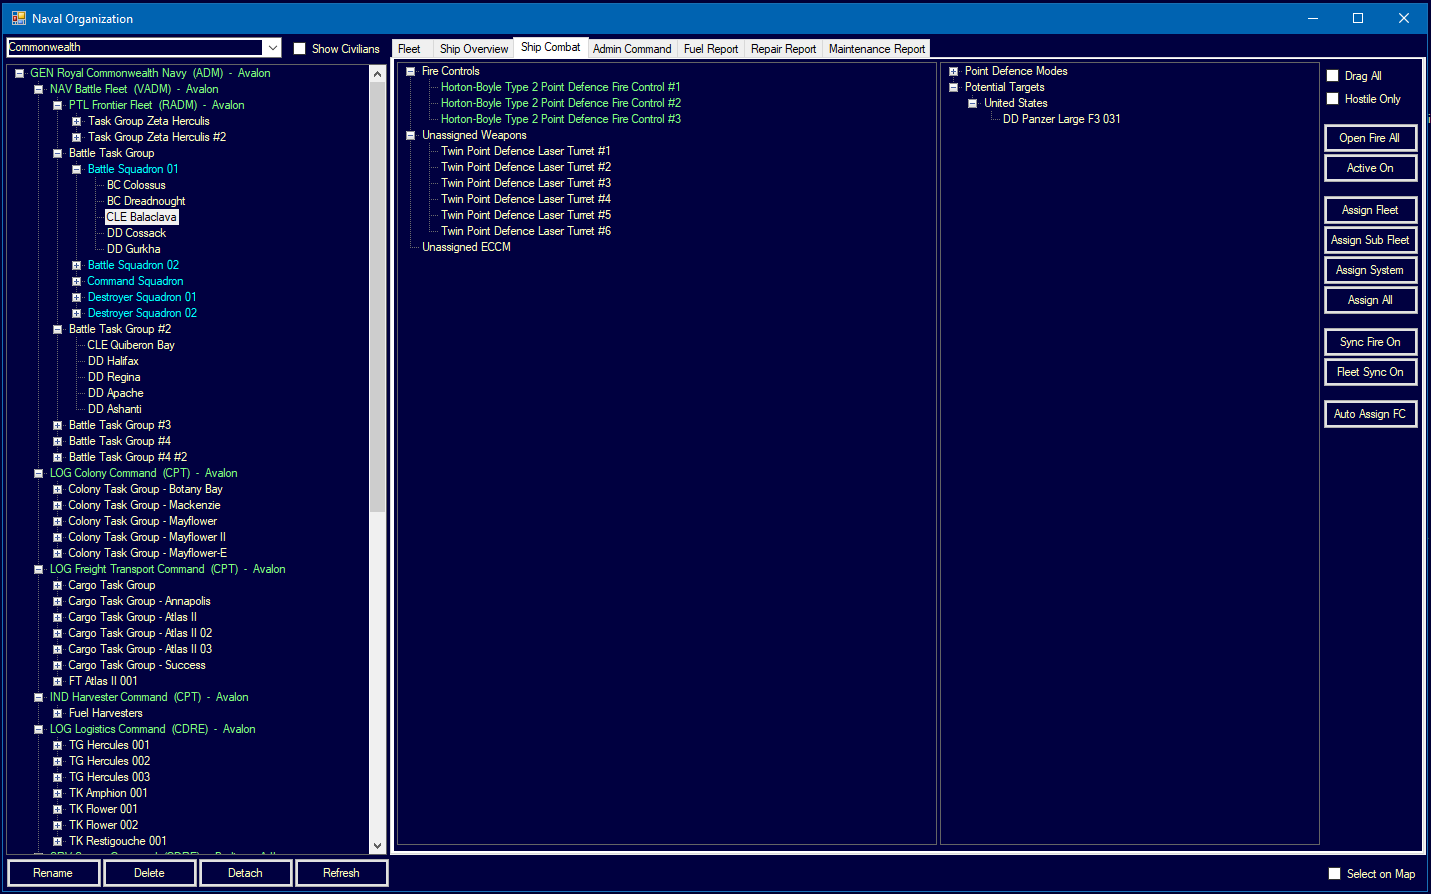
\includegraphics[width=0.95\linewidth]{images/AutomatedAssignment}
		\caption[Automated Assignment]{Automated Assignment Example 1}
		\label{fig:automatedassignment}
	\end{figure}
	\begin{figure}[H]
		\centering
		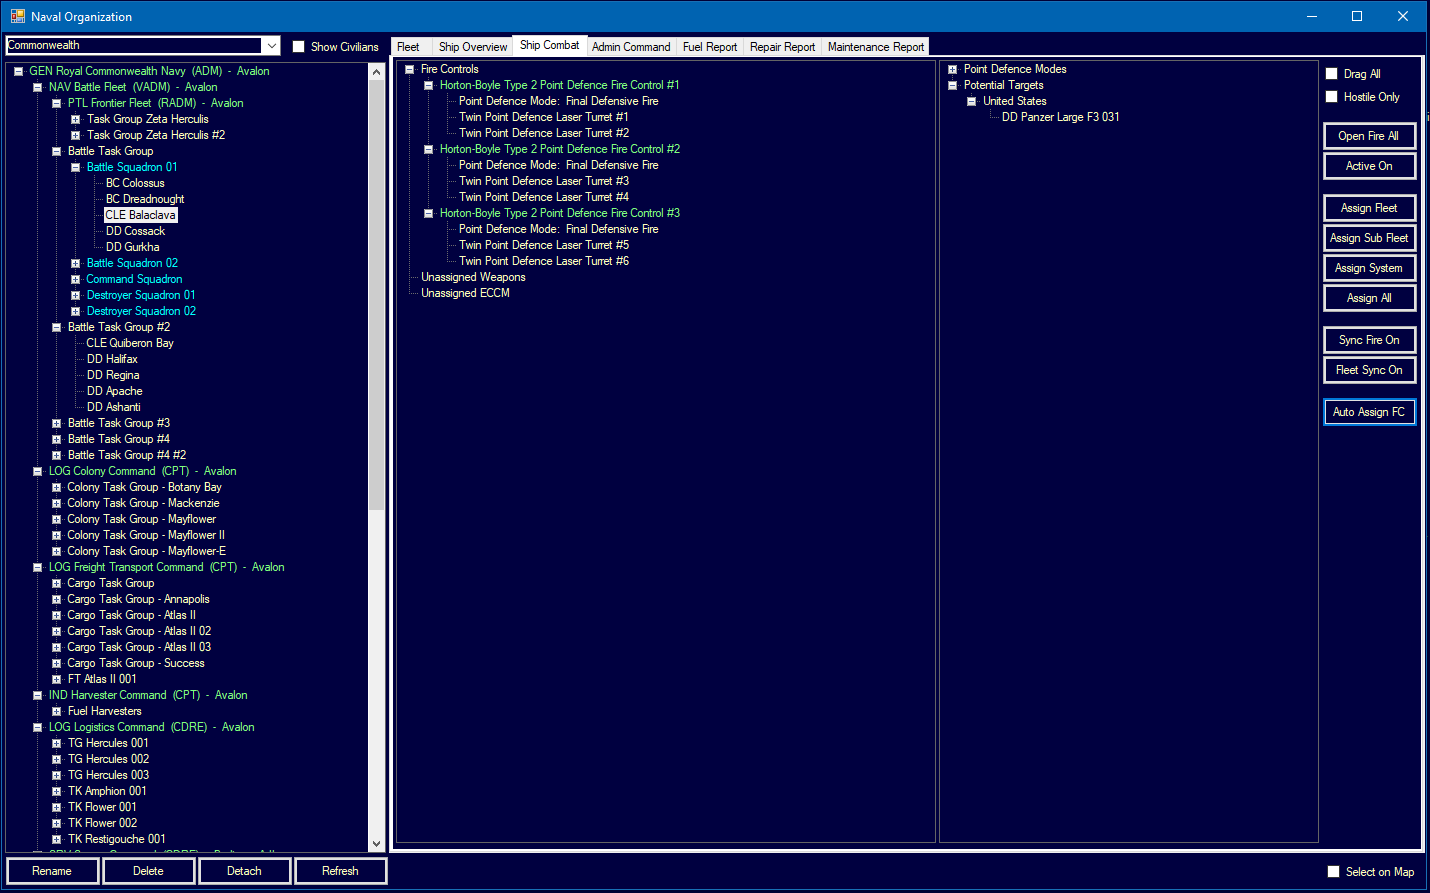
\includegraphics[width=0.95\linewidth]{images/AutomatedAssignment2}
		\caption[Automated Assignment]{Automated Assignment Example 2}
		\label{fig:automatedassignment2}
	\end{figure}
	
	This ship has a mixture of point defence and offensive lasers, plus fire controls for each. The auto-assign determines which weapons should be assigned to which fire control. All beam fire control are set as final fire so the ship will use all available weapons to defend against missile attack.
	\begin{figure}[H]
		\centering
		\begin{subfigure}{.5\textwidth}
			\centering
			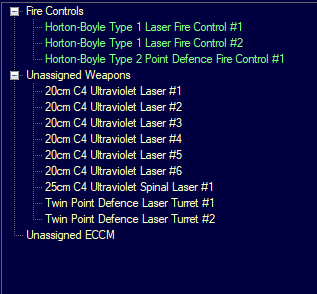
\includegraphics[width=0.5\linewidth]{images/AutomatedAssignment3}
			\caption[Automated Assignment]{Automated Assignment Example 3}
			\label{fig:automatedassignment3}
		\end{subfigure}%
		\begin{subfigure}{.5\textwidth}
			\centering
			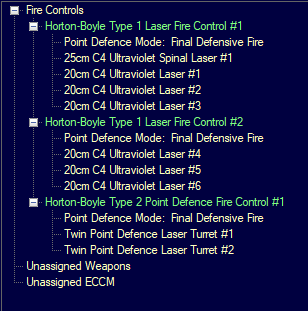
\includegraphics[width=0.5\linewidth]{images/AutomatedAssignment4}
			\caption[Automated Assignment]{Automated Assignment Example 4}
			\label{fig:automatedassignment4}
		\end{subfigure}
	\end{figure}

	This ship has a mixture of missiles and offensive lasers. Note that missiles are automatically assigned to launchers.
	\begin{figure}[H]
		\centering
		\begin{subfigure}{.5\textwidth}
			\centering
			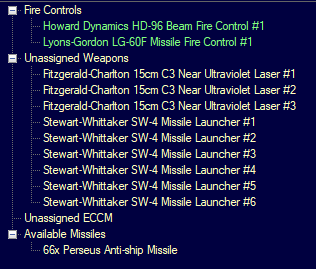
\includegraphics[width=0.5\linewidth]{images/AutomatedAssignment5}
			\caption[Automated Assignment]{Automated Assignment Example 5}
			\label{fig:automatedassignment5}
		\end{subfigure}%
		\begin{subfigure}{.5\textwidth}
			\centering
			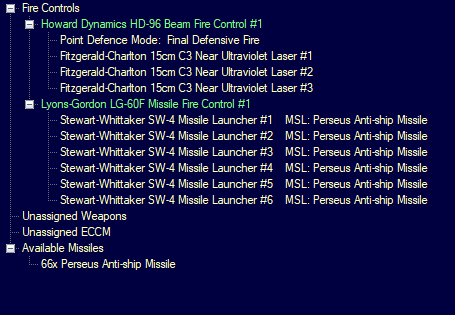
\includegraphics[width=0.5\linewidth]{images/AutomatedAssignment6}
			\caption[Automated Assignment]{Automated Assignment Example 6}
			\label{fig:automatedassignment6}
		\end{subfigure}
	\end{figure}
	
	This ship has a point defence turret and multiple types of offensive beam weapons, plus an ECCM system.
	\begin{figure}[H]
		\centering
		\begin{subfigure}{.5\textwidth}
			\centering
			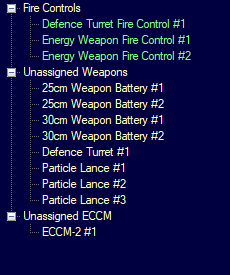
\includegraphics[width=0.5\linewidth]{images/AutomatedAssignment7}
			\caption[Automated Assignment]{Automated Assignment Example 7}
			\label{fig:automatedassignment7}
		\end{subfigure}%
		\begin{subfigure}{.5\textwidth}
			\centering
			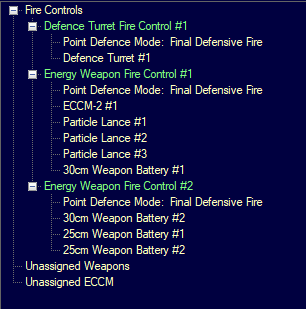
\includegraphics[width=0.5\linewidth]{images/AutomatedAssignment8}
			\caption[Automated Assignment]{Automated Assignment Example 8}
			\label{fig:automatedassignment8}
		\end{subfigure}
	\end{figure}

	An extreme example!
	\begin{figure}[H]
		\centering
		\begin{subfigure}{.5\textwidth}
			\centering
			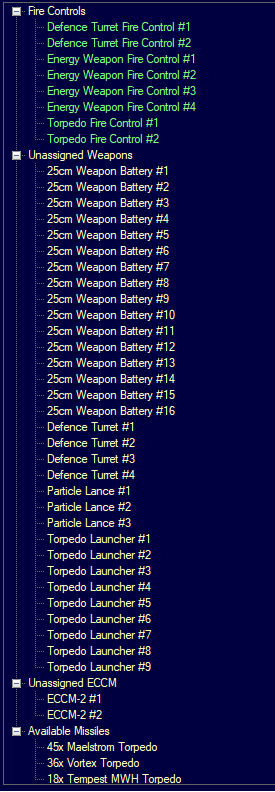
\includegraphics[width=0.5\linewidth]{images/AutomatedAssignment9}
			\caption[Automated Assignment]{Automated Assignment Example 9}
			\label{fig:automatedassignment9}
		\end{subfigure}%
		\begin{subfigure}{.5\textwidth}
			\centering
			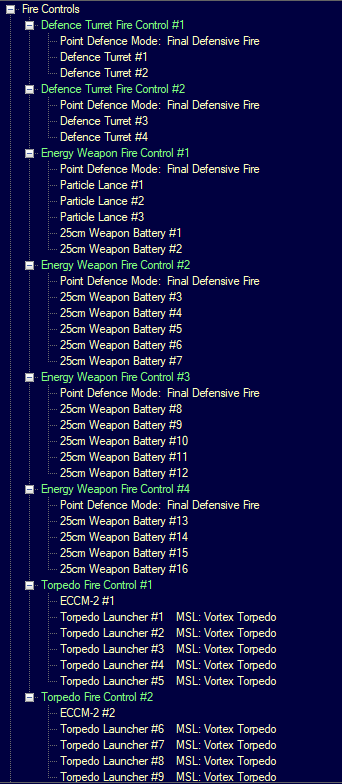
\includegraphics[width=0.5\linewidth]{images/AutomatedAssignment10}
			\caption[Automated Assignment]{Automated Assignment Example 10}
			\label{fig:automatedassignment10}
		\end{subfigure}
	\end{figure}


	\subsection{Atmoshpere and energy weapons}
	Original post can be found
	\href{http://aurora2.pentarch.org/index.php?topic=8495.msg107702#msg107702}{here}.
	\\\\
	
	In C\# Aurora, there is no penalty for energy weapons firing in or through an atmosphere.
	
	
	\subsection{Planetary bombardment}
	Original post can be found
	\href{http://aurora2.pentarch.org/index.php?topic=8495.msg107703#msg107703}{here}.
	\\\\
	
	In C\# Aurora, populations can be attacked by missiles and energy weapons. However, because missile warheads are area-effect weapons, they are much more effective at destroying the civilian population and any installations.
	
	Each installation type has a Target Size. The chance of each attack (either a missile or a single energy weapon) destroying an installation is equal to: Weapon Damage / Target Size. For example, a construction factory has a Target Size of 20, so a 10cm laser fired from orbit would have a 15\% chance to destroy the target (3 / 20). For the purposes of this check, missile warheads are treated as equal to 20x warhead strength. Therefore, a single 1 point warhead has a 100\% chance to destroy a construction factory.
	
	A single energy weapon can destroy only one target per hit. A missile warhead is applied until all damage is used. For example, a 5-point missile warhead is counted as 100. If the first installation hit is a construction factory, that factory is destroyed and the remaining damage reduced to 80. That damage is then applied the next installation hit and so on.
	
	Missile warheads cause radiation and dust levels to increase by an amount equal to their warhead size. Energy weapons increase the dust level by 5\% of their damage amount.
	
	Missile warheads inflict civilian casualties at the rate of 100,000 per point of damage. Energy weapons inflict civilian casualties at the rate of 2,000 per point of damage.
	
	Populations will no longer surrender purely due to orbital bombardment. You have to land ground formations to force a surrender.
	
	Energy weapons now provide a way to destroy the industry and infrastructure of a target population, without causing radiation or using up ordnance. However, this will require considerable effort for a large population and consume maintenance supplies due to weapon failures. It will also bring you within range of any ground-based energy weapons. Of course, it will usually be more beneficial to conquer the planet and gain the installations instead of destroying them.
	
	\begin{center}
		\begin{tabular}{|l|r|}
			\hline
			\textbf{Name} & \textbf{Target size} \\
			\hline
			Automated Mine & 20 \\
			\hline
			Cargo Shuttle Station & 200 \\
			\hline
			Civilian Mining Complex & 200 \\
			\hline
			Construction Factory & 20 \\
			\hline
			Conventional Industry & 20 \\
			\hline
			Deep Space Tracking Station & 40 \\
			\hline
			Fighter Factory & 20 \\
			\hline
			Financial Centre & 20 \\
			\hline
			Forced Labour Construction Camp & 80 \\
			\hline
			Forced Labour Mining Camp & 80 \\
			\hline
			Fuel Refinery & 20 \\
			\hline
			Genetic Modification Centre & 400 \\
			\hline
			Ground Force Training Facility & 400 \\
			\hline
			Infrastructure & 2 \\
			\hline
			Low Gravity Infrastructure & 2 \\
			\hline
			Maintenance Facility & 20 \\
			\hline
			Mass Driver & 20 \\
			\hline
			Military Academy & 400 \\
			\hline
			Mine & 20 \\
			\hline
			Naval Headqarters & 400 \\
			\hline
			Ordnance Factory & 20 \\
			\hline
			Ordnance Transfer Station & 200 \\
			\hline
			Refuelling Station & 200 \\
			\hline
			Research Lab & 400 \\
			\hline
			Sector Command & 400 \\
			\hline
			Spaceport & 1000 \\
			\hline
			Terraforming Installation & 100 \\
			\hline
		\end{tabular}
	\end{center}


\end{document}